\documentclass[fleqn, 11pt]{article}
\usepackage[spanish]{babel}
\usepackage[utf8]{inputenc}
\usepackage{amsmath, amssymb, amsfonts}
\usepackage{parskip}
\usepackage{lipsum}
\usepackage[left = 18mm, right = 18mm, bottom = 18mm, top = 18mm]{geometry}
\usepackage{tcolorbox}
\tcbuselibrary{theorems}
\tcbuselibrary{breakable}
\usepackage{colortbl}
\usepackage{array, tabularx}
\usepackage[pdftex, hidelinks]{hyperref}
\usepackage{multirow}
\usepackage{multicol}
\usepackage{enumerate}
\usepackage{graphicx}

\usepackage[proportional,scaled=1.064]{erewhon}
\usepackage[erewhon,vvarbb,bigdelims]{newtxmath}
\usepackage[T1]{fontenc}
\renewcommand*\oldstylenums[1]{\textosf{#1}}

\newcommand{\gradial}{\hspace{0.9mm} 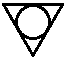
\includegraphics[width = 3mm]{gradial.png} \hspace{1mm}}

\tcbsetforeverylayer{autoparskip}

\tcbset{theorem full label supplement={hypertarget={#1}}}

\newtcbtheorem[auto counter, number freestyle = {\noexpand \arabic{\tcbcounter}}]{definicion}{D\hspace{0.1mm}e\hspace{0.1mm}f\hspace{0.4mm}i\hspace{0.1mm}n\hspace{0.1mm}i\hspace{0.1mm}c\hspace{0.1mm}i\hspace{0.1mm}ó\hspace{0.1mm}n}{colback = white, colframe = black, fonttitle = \bfseries}{def}

\newtcbtheorem[auto counter, number freestyle = {\noexpand \arabic{\tcbcounter}}]{teorema}{T\hspace{0.1mm}e\hspace{0.1mm}o\hspace{0.1mm}r\hspace{0.1mm}e\hspace{0.1mm}m\hspace{0.1mm}a}{colback = white, colframe = black, fonttitle = \bfseries}{teo}

\newtcbtheorem[use counter from = teorema]{proposicion}{P\hspace{0.1mm}r\hspace{0.1mm}o\hspace{0.1mm}p\hspace{0.1mm}o\hspace{0.1mm}s\hspace{0.1mm}i\hspace{0.1mm}c\hspace{0.1mm}i\hspace{0.1mm}ó\hspace{0.1mm}n}{colback = white, colframe = black, fonttitle = \bfseries}{prop}

\newtcbtheorem[use counter from = teorema]{corolario}{C\hspace{0.1mm}o\hspace{0.1mm}r\hspace{0.1mm}o\hspace{0.1mm}l\hspace{0.1mm}a\hspace{0.1mm}r\hspace{0.1mm}i\hspace{0.1mm}o}{colback = white, colframe = black, fonttitle = \bfseries}{cor}

\newtcbtheorem[use counter from = teorema]{lema}{L\hspace{0.1mm}e\hspace{0.1mm}m\hspace{0.1mm}a}{colback = white, colframe = black, fonttitle = \bfseries}{lem}

\newtcbtheorem[auto counter, number freestyle = {\noexpand \arabic{\tcbcounter}}]{ejemplo}{E\hspace{0.1mm}j\hspace{0.1mm}e\hspace{0.1mm}m\hspace{0.1mm}p\hspace{0.1mm}l\hspace{0.1mm}o}{colback = white, colframe = black, fonttitle = \bfseries}{ejem}

\begin{document}
    \begin{definicion}[beforeafter skip = 4mm]{}{grafica_de_grados}
        Sean $ G_1 $ y $ G_2 $ gráficas tales que $ \textnormal{V}(G_1) \cap \textnormal{V}(G_2) = \emptyset $. Se define a $ G_1 \gradial G_2 = (\textnormal{V}, \textnormal{A}) $ como la \textbf{gráfica gradial de $ G_1 $ y $ G_2 $} con \vspace{2mm}
        
        $ \textnormal{V}(G_1 \gradial G_2) = \textnormal{V}(G_1) \cup \textnormal{V}(G_2) $ \quad y \vspace{-1mm}
        \begin{align*}
            \hspace{-9mm} \textnormal{A}(G_1 \gradial G_2) =& \left\{ uv \mid u \in \textnormal{V}(G_1), \, v \in \textnormal{V}(G_2), \textnormal{ gr}(u) = \delta(G_1) + l \phantom{|_i^i} \textnormal{y} \phantom{|_i^i} \textnormal{gr}(v) = \Delta(G_2) - l, \right. \\
            & \left. \phantom{|_i^i} \textnormal{con } l = 0,1, \ldots, \lvert \textnormal{V}(G_2) \rvert \right\} \cup  \left\{ uv \mid u \in \textnormal{V}(G_2), \, v \in \textnormal{V}(G_1), \textnormal{ gr}(u) = \delta(G_2) + l \phantom{|_i^i} \textnormal{y } \right. \\
            & \left. \phantom{|_i^i} \textnormal{gr}(v) = \Delta(G_1) - l, \textnormal{ con } l = 0,1, \ldots, \lvert \textnormal{V}(G_1) \rvert \right\}
        \end{align*}
    \end{definicion}

    \begin{ejemplo}[breakable, pad at break = 4mm, beforeafter skip = 3mm]{}{procedimiento_construccion_Gg}
        Sean $ G_1 $ y $ G_2 $ gráficas como se muestra abajo. Para construir la gráfica de grados de $ G_1 $ y $ G_2 $, se puede seguir el siguiente procedimiento: \vspace{3mm}

        \begin{center}
            \begin{minipage}[h]{0.3\linewidth}
                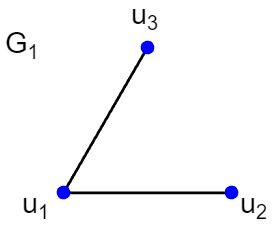
\includegraphics[width=0.9\linewidth]{Ejemplo_1/Ejemplo1_G1.jpg}
            \end{minipage} \hspace{0.1\linewidth}
            \begin{minipage}[h]{0.3\linewidth}
                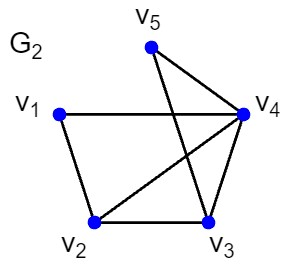
\includegraphics[width=0.9\linewidth]{Ejemplo_1/Ejemplo1_G2.jpg}
            \end{minipage}
        \end{center} \vspace{3mm}

        \begin{enumerate}
            \item Obtener el grado máximo y mínimo de cada gráfica. En este caso, $ \delta(G_1) = 1, \delta(G_2) = 2 $, \mbox{$ \Delta(G_1) = 2 $} y $ \Delta(G_2) = 4 $. \vspace{3mm}
            \item Elaborar dos tablas donde la primer fila esté conformada por los grados anteriormente obtenidos como se muestra a continuación: \vspace{3mm}
            
            \begin{center}
                \begin{minipage}[h]{0.3\linewidth}
                    \begin{tcolorbox}[title empty, center, colframe = black!99!white, colback = white, sharp corners, hbox, left = -0.9mm, right = -0.9mm, top = -0.9mm, bottom = -0.9mm]
                        \begin{tabular}{c|c}
                            \rowcolor{gray!36!white} 
                            $ \delta(G_1) = 1 $ & $ \Delta(G_2) = 4 $ 
                        \end{tabular}
                    \end{tcolorbox}
                \end{minipage}
                \begin{minipage}[h]{0.3\linewidth}
                    \begin{tcolorbox}[title empty, center, colframe = black!99!white, colback = white, sharp corners, hbox, left = -0.9mm, right = -0.9mm, top = -0.9mm, bottom = -0.9mm]
                        \begin{tabular}{c|c}
                            \rowcolor{gray!36!white} 
                            $ \delta(G_2) = 2 $ & $ \Delta(G_1) = 2 $ 
                        \end{tabular}
                    \end{tcolorbox}
                \end{minipage}
            \end{center} \vspace{3mm}
            
            \item En las columnas de las tablas que corresponden a los grados máximos de cada gráfica, se coloca el número de la celda anterior disminuido en uno, hasta llegar al cero. Mientras que las columnas que corresponden a los grados mínimos se coloca el número de la celda anterior aumentado en uno. \vspace{3mm}
            
            \begin{center}
                \begin{minipage}[h]{0.3\linewidth}
                    \begin{tcolorbox}[title empty, center, colframe = black!99!white, colback = white, sharp corners, hbox, nobeforeafter, left = -0.9mm, right = -0.9mm, top = -0.9mm, bottom = -0.9mm]
                        \begin{tabular}{c|c}
                            \rowcolor{gray!36!white} 
                            $ \delta(G_1) = 1 $ & $ \Delta(G_2) = 4 $ \\ \hline\hline
                            $ 2 $               & $ 3 $ \\ \hline
                            $ 3 $               & $ 2 $ \\ \hline
                            $ 4 $               & $ 1 $ \\ \hline
                            $ 5 $               & $ 0 $
                        \end{tabular}
                    \end{tcolorbox}
                \end{minipage}
                \begin{minipage}[h]{0.3\linewidth}
                    \begin{tcolorbox}[title empty, center, colframe = black!99!white, colback = white, sharp corners, hbox, nobeforeafter, left = -0.9mm, right = -0.9mm, top = -0.9mm, bottom = -0.9mm]
                        \begin{tabular}{c|c}
                            \rowcolor{gray!36!white} 
                            $ \delta(G_2) = 2 $ & $ \Delta(G_1) = 2 $ \\ \hline\hline
                            $ 3 $               & $ 1 $ \\ \hline
                            $ 4 $               & $ 0 $
                        \end{tabular}
                    \end{tcolorbox}
                \end{minipage}
            \end{center} \vspace{3mm}

            \item Por último, se dibujan los vértices de ambas gráficas y se hacen adyacentes aquellos que tengan el grado indicado en cada fila, en su respectiva gráfica.
            
            \begin{center}
                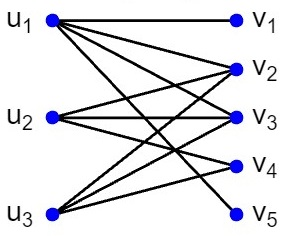
\includegraphics[width=0.3\linewidth]{Ejemplo_1/Ejemplo1_Gg.jpg}
            \end{center}
        \end{enumerate}
    \end{ejemplo}

    Por cómo se definió la gráfica de grados, es claro que ningún par de vértices de cada una de las dos gráficas que la definen son adyacentes entre sí. Esto da lugar a la siguiente proposición.

    \begin{proposicion}[beforeafter skip = 4mm]{}{Gg_bipartita}
        Si $ G_1 $ y $ G_2 $ son gráficas, entonces $ G_1 \ast G_2 $ es bipartita.
    \end{proposicion}

    \textbf{Observación.} Ya que la gráfica de grados es bipartita, su número cromático es 2.

    \begin{proposicion}[beforeafter skip = 4mm]{}{conmutatividad}
            Si $ G_1 $ y $ G_2 $ son gráficas, entonces $ G_1 \ast G_2 = G_2 \ast G_1 $.
    \end{proposicion}

    En los próximos enunciados se pueden atribuir propiedades concretas a las gráficas que definen la gráfica de grados. Debido a la Proposición \eqref{prop:conmutatividad}, estas propiedades también se le pueden atribuir a la otra gráfica.

    \begin{teorema}[beforeafter skip = 4mm]{}{subgrafica_bipartita_completa}
        Sean $ G_1 $ y $ G_2 $ gráficas tal que $ G_1 $ es $ r $-regular. Si $ V' = \left\lbrace v \in \textnormal{V}(G_2) \mid \textnormal{gr}(v) = \delta(G_2) \textnormal{ gr}(v) = \Delta(G_2) \right\rbrace $, entonces \vspace{3mm}
        
        \begin{enumerate}[i)]
            \item la subgráfica inducida de $ G_1 \ast G_2 $ por $ \textnormal{V}(G_1) \cup V' $ es bipartita completa.
            \item Todo $ v \in \textnormal{V}(G_2) \setminus V' $ es aislado.
        \end{enumerate}
    \end{teorema}

    \begin{corolario}[beforeafter skip = 4mm]{}{maxmin_bipartita_completa}
        Sean $ G_1 $ y $ G_2 $ gráficas. Si $ G_1 $ es $ r $-regular y para todo $ v \in \textnormal{V}(G_2) $ se da que gr$(v) = \delta(G_2) $ ó gr$(v) = \Delta(G_2) $, entonces $ G_1 \ast G_2 $ es bipartita completa.
    \end{corolario}

    \begin{corolario}[beforeafter skip = 4mm]{}{regulares_completa}
        Si $ G_1 $ y $ G_2 $ son gráficas $ r $-regular y $ s $-regular, respectivamente, entonces $ G_1 \ast G_2 $ es bipartita completa.
    \end{corolario}

    \textbf{Observaciones.}

    \begin{enumerate}
        \item $ K_n \ast K_m $ es bipartita completa $ \forall n, m \in \mathbb{N} $, pues $ K_n $ y $ K_m $ son $ (n-1) $-regular y $ (m-1) $-regular, respectivamente.
        \item $ C_n \ast C_m $ es bipartita completa $ \forall n, m \in \mathbb{N} $, pues $ C_n $ y $ C_m $ son gráficas $ 2 $-regular.
    \end{enumerate} \vspace{1mm}

    \begin{proposicion}[beforeafter skip = 4mm]{}{menos_procedimiento}
        Sean $ G_1 $ y $ G_2 $ gráficas. Si $ \delta(G_1) + \Delta(G_2) = \delta(G_2) + \Delta(G_1) $ entonces \begin{align*}
            \textnormal{A}(G_1 \ast G_2) &= \left\{ uv \mid u \in \textnormal{V}(G_1), \, v \in \textnormal{V}(G_2), \textnormal{ gr}(u) = \delta(G_1) + l \phantom{|_i^i} \textnormal{y} \phantom{|_i^i} \textnormal{gr}(v) = \Delta(G_2) - l, \textnormal{ con } \right. \\
            & \left. \quad \phantom{|_i^i} l = 0,1, \ldots, \lvert \textnormal{V}(G_2) \rvert \right\} \\
            &= \left\{ uv \mid u \in \textnormal{V}(G_2), \, v \in \textnormal{V}(G_1), \textnormal{ gr}(u) = \delta(G_2) + l \phantom{|_i^i} \textnormal{y} \phantom{|_i^i} \textnormal{gr}(v) = \Delta(G_1) - l, \textnormal{ con } \right. \\
            & \left. \quad \phantom{|_i^i} l = 0,1, \ldots, \lvert \textnormal{V}(G_1) \rvert \right\}
        \end{align*}
    \end{proposicion}

    Si dos gráficas cumplen la hipótesis de la Proposición \eqref{prop:menos_procedimiento}, entonces solo es necesario seguir el procedimiento del Ejemplo \eqref{ejem:procedimiento_construccion_Gg}, pero con solo una de las dos tablas, para construir la gráfica de grados de ambas gráficas.

    \begin{teorema}[beforeafter skip = 4mm]{}{Gg_igual_complementos}
        Si $ G_1 $ y $ G_2 $ son gráficas, entonces $ G_1 \ast G_2 = G_1^C \ast G_2^C $.
    \end{teorema}

    \begin{teorema}[beforeafter skip = 4mm]{}{trayectoria_minima}
        Sean $ G_1 $ y $ G_2 $ gráficas. Si para $ u,v \in \textnormal{V}(G_1) $ existe una $ uv $-trayectoria en $ G_1 \ast G_2 $ entonces existe una $ uv $-trayectoria $ T $ en $ G_1 \ast G_2 $ de longitud 2, con $ T = (u,w,v) $ donde $ w \in \textnormal{V}(G_2) $.
    \end{teorema}

    \begin{teorema}[beforeafter skip = 4mm]{}{disconexidad_igualdad_grados}
        Sean $ G_1 $ y $ G_2 $ gráficas, con $ G_1 $ disconexa. Si $ \delta(G_1) = \delta(G_2) < \Delta(G_1) = \Delta(G_2) $ entonces $ G_1 \ast G_2 $ es disconexa.
    \end{teorema}

    \begin{teorema}[beforeafter skip = 4mm]{}{graficas_isomorfas}
        Si $ G_1 $ y $ G_2 $ son gráficas no regulares tales que $ G_1 \cong G_2 $, entonces \vspace{3mm}

        \begin{tabular}{rl}
            
        \end{tabular}

        \begin{enumerate}
            \item $ \textnormal{A}(G_1 \ast G_2) = \left\{ uv \mid u \in \textnormal{V}(G_1), \, v \in \textnormal{V}(G_2), \textnormal{ gr}(u) = \delta(G_1) + l \phantom{|_i^i} \textnormal{y} \phantom{|_i^i} \textnormal{gr}(v) = \Delta(G_2) - l, \right. $
            $ \left. \textnormal{ con } \phantom{|_i^i} l = 0,1, \ldots, \lvert \textnormal{V}(G_2) \rvert \right\} $

            $ \left\{ uv \mid u \in \textnormal{V}(G_2), \, v \in \textnormal{V}(G_1), \textnormal{ gr}(u) = \delta(G_2) + l \phantom{|_i^i} \textnormal{y} \phantom{|_i^i} \textnormal{gr}(v) = \Delta(G_1) - l, \textnormal{ con } \right. $
            $ \left. \quad \phantom{|_i^i} l = 0,1, \ldots, \lvert \textnormal{V}(G_1) \rvert \right\} $
            
            \item $ G_1 \ast G_2 $ es disconexa.
        \end{enumerate}
    \end{teorema}
\end{document}